\documentclass[tikz,border=8pt]{standalone}
\usepackage{tikz}
\usetikzlibrary{positioning,arrows.meta,shapes.geometric,fit,backgrounds}

\begin{document}
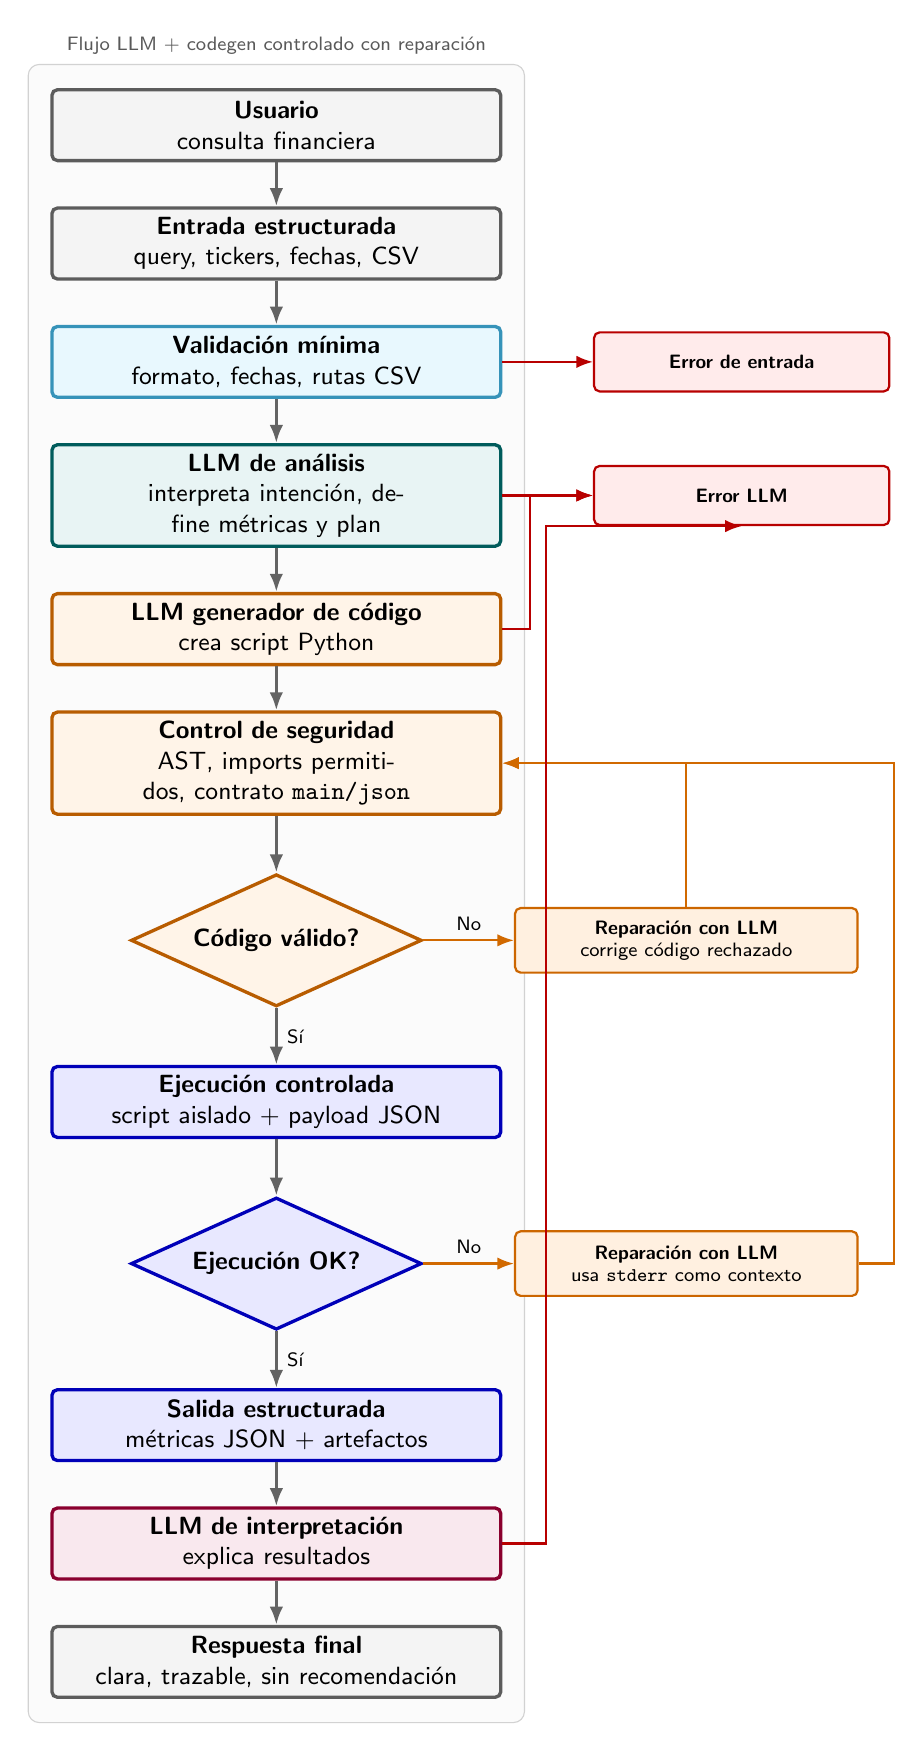
\begin{tikzpicture}[
    font=\sffamily\small,
    node distance=0.56cm,
    step/.style={
        draw=#1!72!black,
        fill=#1!9,
        rounded corners=2pt,
        very thick,
        align=center,
        minimum width=5.7cm,
        minimum height=0.9cm,
        text width=5.25cm
    },
    decision/.style={
        diamond,
        draw=#1!72!black,
        fill=#1!9,
        very thick,
        align=center,
        aspect=2.2,
        inner sep=1pt,
        text width=2.85cm
    },
    error/.style={
        draw=red!72!black,
        fill=red!8,
        rounded corners=2pt,
        thick,
        align=center,
        minimum width=3.75cm,
        minimum height=0.75cm,
        text width=3.45cm,
        font=\sffamily\scriptsize
    },
    repair/.style={
        draw=orange!80!black,
        fill=orange!12,
        rounded corners=2pt,
        thick,
        align=center,
        minimum width=4.35cm,
        minimum height=0.82cm,
        text width=4.0cm,
        font=\sffamily\scriptsize
    },
    arrow/.style={-{Latex[length=2.3mm]}, very thick, draw=gray!78!black},
    errorarrow/.style={-{Latex[length=2.1mm]}, thick, draw=red!72!black},
    repairarrow/.style={-{Latex[length=2.1mm]}, thick, draw=orange!82!black}
]

\node[step=gray] (user) {\textbf{Usuario}\\consulta financiera};
\node[step=gray, below=of user] (input) {\textbf{Entrada estructurada}\\query, tickers, fechas, CSV};
\node[step=cyan, below=of input] (validation) {\textbf{Validaci\'on m\'inima}\\formato, fechas, rutas CSV};
\node[step=teal, below=of validation] (analysis) {\textbf{LLM de an\'alisis}\\interpreta intenci\'on, define m\'etricas y plan};
\node[step=orange, below=of analysis] (codegen) {\textbf{LLM generador de c\'odigo}\\crea script Python};
\node[step=orange, below=of codegen] (security) {\textbf{Control de seguridad}\\AST, imports permitidos, contrato \texttt{main/json}};
\node[decision=orange, below=0.72cm of security] (valid) {\textbf{C\'odigo v\'alido?}};
\node[step=blue, below=0.72cm of valid] (execution) {\textbf{Ejecuci\'on controlada}\\script aislado + payload JSON};
\node[decision=blue, below=0.72cm of execution] (execok) {\textbf{Ejecuci\'on OK?}};
\node[step=blue, below=0.72cm of execok] (output) {\textbf{Salida estructurada}\\m\'etricas JSON + artefactos};
\node[step=purple, below=of output] (interpretation) {\textbf{LLM de interpretaci\'on}\\explica resultados};
\node[step=gray, below=of interpretation] (final) {\textbf{Respuesta final}\\clara, trazable, sin recomendaci\'on};

\node[repair, right=1.15cm of valid] (repairsecurity) {\textbf{Reparaci\'on con LLM}\\corrige c\'odigo rechazado};
\node[repair, right=1.15cm of execok] (repairexec) {\textbf{Reparaci\'on con LLM}\\usa \texttt{stderr} como contexto};

\node[error, right=1.15cm of validation] (inputerror) {\textbf{Error de entrada}};
\node[error, right=1.15cm of analysis] (llmerror) {\textbf{Error LLM}};

\draw[arrow] (user) -- (input);
\draw[arrow] (input) -- (validation);
\draw[arrow] (validation) -- (analysis);
\draw[arrow] (analysis) -- (codegen);
\draw[arrow] (codegen) -- (security);
\draw[arrow] (security) -- (valid);
\draw[arrow] (valid) -- node[right, font=\sffamily\scriptsize] {S\'i} (execution);
\draw[arrow] (execution) -- (execok);
\draw[arrow] (execok) -- node[right, font=\sffamily\scriptsize] {S\'i} (output);
\draw[arrow] (output) -- (interpretation);
\draw[arrow] (interpretation) -- (final);

\draw[repairarrow] (valid.east) -- node[above, font=\sffamily\scriptsize] {No} (repairsecurity.west);
\draw[repairarrow] (repairsecurity.north) |- (security.east);
\draw[repairarrow] (execok.east) -- node[above, font=\sffamily\scriptsize] {No} (repairexec.west);
\draw[repairarrow] (repairexec.east) -- ++(0.45,0) |- (security.east);

\draw[errorarrow] (validation.east) -- (inputerror.west);
\draw[errorarrow] (analysis.east) -- (llmerror.west);
\draw[errorarrow] (codegen.east) -- ++(0.35,0) |- (llmerror.west);
\draw[errorarrow] (interpretation.east) -- ++(0.55,0) |- (llmerror.south);

\begin{scope}[on background layer]
\node[
    draw=gray!35,
    fill=gray!3,
    rounded corners=4pt,
    inner xsep=0.28cm,
    inner ysep=0.30cm,
    fit=(user)(input)(validation)(analysis)(codegen)(security)(valid)(execution)(execok)(output)(interpretation)(final),
    label={[font=\sffamily\scriptsize, gray!70!black]above:Flujo LLM + codegen controlado con reparaci\'on}
] {};
\end{scope}

\end{tikzpicture}
\end{document}
